\begin{defnbox}\nospacing
  \begin{defn}[Resolution]
    Is a rule of inference.
  \end{defn}
\end{defnbox}
\begin{defnbox}\nospacing
  \begin{defn}[Type]\label{defn:Type}
    defines a behavior but no implementation.\\
    (Java: Types are defined by classes)
  \end{defn}
\end{defnbox}
\begin{defnbox}\nospacing
  \begin{defn}[Subtyping]\label{defn:}
    Are specializations of Types and define a \rd{is-a} relationship.\\
    (Java: Subtyping is defined by subclassing, i.e. each subclass also defines a subtype)
  \end{defn}
\end{defnbox}
\begin{defnbox}\nospacing
  \begin{defn}[Java Method Signature]\label{defn:}
    Is the method name and the number, type and order of its parameters:
    \begin{mintlinebox}{java}
      methodName(Type1, Type2,...)
    \end{mintlinebox}
  \end{defn}
\end{defnbox}
\begin{notebox}[Note]\nospacing
  Return types, name of the arguments and thrown exceptions are not considered to be a part of the method signature. 
\end{notebox}
\begin{defnbox}\nospacing
  \begin{defn}[Method Declaration]\label{defn:methodDeclaration}
  Is a declaration of a function i.e.\ declares an identifier and its types,\ldots
    \begin{mintlinebox}{java}
      visibility |\optal|static|\optar| returnType methodName (args);
    \end{mintlinebox}
  \end{defn}
\end{defnbox}
\begin{defnbox}\nospacing
  \begin{defn}[Private]\label{defn:private}
    Methods, variables, and constructors that are declared private can only be
    accessed within the declared class itself.\\
    A \textit{subclass} does not inherit the private members of its parent
    class.
    Private means you can Only access it in that class an no where else.\\
    However, if the superclass has public or protected methods for accessing its
    private fields, these can also be used by the subclass.
  \end{defn}
\end{defnbox}
\begin{consequencebox}[Consequence]\nospacing
  Methods declared private are not inherited at all.
\end{consequencebox}

\begin{notebox}[Note: nested classes]\nospacing
  A nested class has access to all the private members of its enclosing class—both fields and methods.
\end{notebox}
\begin{defnbox}\nospacing
  \begin{defn}[Public]\label{defn:private}
    A class, method, constructor, interface, etc.\ declared public can be
    accessed from any class belonging to the Java universe.
  \end{defn}
\end{defnbox}
\begin{consequencebox}[Consequence]\nospacing
  \begin{itemizenosep}
      \item Methods declared public in a superclass also must be public in all subclasses
  \end{itemizenosep}
\end{consequencebox}
\begin{defnbox}\nospacing
  \begin{defn}[Protected]\label{defn:protected}
    Variables, methods, and constructors, which are declared protected in a superclass can be accessed only by the subclasses in other package or any class within the package of the protected members' class.
  \end{defn}
\end{defnbox}
\begin{consequencebox}[Consequence]\nospacing
  \begin{itemizenosep}
    \item
Methods declared protected in a superclass must either be protected or public in
subclasses; they cannot be private.
\end{itemizenosep}
\end{consequencebox}
\begin{consequencebox}[Consequence]\nospacing
    Only \javainline{protected} and \javainline{public} methods/variables can
    be inherited and/or overridden $\iff$
    Subclasses can only invoke or override \javainline{protected} or \javainline{public} methods.
\end{consequencebox}
\begin{notebox}[Note: methods without access modifiers]\nospacing
  Can be overridden, if the superclass is in the same package.
\end{notebox}
\begin{defnbox}\nospacing
  \begin{defn}[\javainline{final} variables]\label{defn:finalVar}
    A final variable can only be assigned once (final assignment) and will
    always have the same reference hence:
    \begin{mintlinebox}{java}
      final var1 = 5; // or
      final var2;
      var = 5;
    \end{mintlinebox}
    \begin{itemizenosep}
        \item If a final variable is assigned to a primitive, then the value of
        the variable will be constant.
        \item If a final variable holds a reference to an object, then the state
        of the object may still change, but the viable will always refer to the
        same object = \rdb{non-transitivity}
    \end{itemizenosep}
  \end{defn}
\end{defnbox}
\begin{notebox}[Note]\nospacing
  Non-transitivity also applies to arrays, as arrays are mutable i.e.\ we can change
  the elements of the array.
\end{notebox}
\begin{defnbox}\nospacing
  \begin{defn}[\javainline{final} methods]\label{defn:finalMethods}
    A final method cannot be overridden or hidden by subclasses
    This is used to prevent unexpected behavior from a subclass e.g.\
    altering a method that may be crucial to the function or consistency of the class.
  \end{defn}
\end{defnbox}
\begin{defnbox}\nospacing
  \begin{defn}[\javainline{final} Classes]\label{defn:finalClasses}
  A final class cannot be subclassed/extended.
  \end{defn}
\end{defnbox}
\begin{notebox}[Note]\nospacing
  Doing this can confer security and efficiency benefits thus
  many of the Java standard library classes are final.
\end{notebox}
\subsubsection{Mutable Types}
\label{subsubsec:MutableTypes}
\begin{defnbox}\nospacing
  \begin{defn}[Mutable Types]\label{defn:Mutable}
    Are types that can be ``mutated''/changed/modified, while
    maintaining its identity/reference\\
    Arrays are mutable $\Rightarrow$ we may not change its reference
    \imp{but} its contents!\\
    \imp{Examples}:
    \begin{itemizenosep}
        \item Lists
        \item Every class whose members can be altered ($\Rightarrow$ a lot)
    \end{itemizenosep}
  \end{defn}
\end{defnbox}
\begin{sectionbox}[Mutable types\&security]\nospacing
  If we simply return a mutable type, clients may alter
  e.g.\ signers (cryptographically signed objects) of objects $\Rightarrow$
  Return copies by:
  \begin{itemizenosep}
      \item Return deep copies using clone:
      \begin{mintlinebox}{java}
        public Rectangle getBounds(){ return (Rectangle) bounds.clone();}
      \end{mintlinebox}
      \item Use copy constructor to return new instance of given type:
      \begin{mintlinebox}{java}
        public Object[] getSigners(){ return new Signers(this) }
      \end{mintlinebox}
  \end{itemizenosep}
\end{sectionbox}
\begin{notebox}[Notes]\nospacing
  \begin{itemizenosep}
      \item Deepcopy and copyconstructor Need to be implemented!
      \item If we do not make a deep copy, mutable types may still
      be altered even if they are private and do not get returned!
  \end{itemizenosep}
\end{notebox}
\begin{figure}[H]
  \centering
  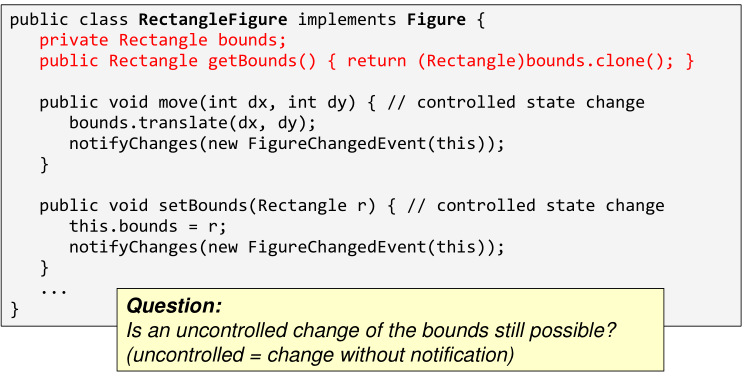
\includegraphics[width=1.0\columnwidth]{figures/uncontrolledChange.png}
  \caption{Uncontrolled changed if clone does not deep copy}
  \label{fig:deepCopy}
\end{figure}
\subsubsection{Immutable Types}
\label{subsubsec:ImmutableTypes}
\begin{defnbox}\nospacing
  \begin{defn}[Immutable Types]\label{defn:Immutable}
    Are types are types whose objects states cannot be modified after
    creation (they can only be in one state).\\
    \imp{Examples}: (\tc{Blue}{Blue} are not \javainline{final})
    \begin{itemizenosep}
      \item java.lang.String
      \item \tc{Blue}{java.awt.Color}
      \item \tc{Blue}{BigInteger}, \tc{Blue}{BigDecimal}, MathContext, 
      \item Character, Boolean, Byte, Double, Float, Integer, Long, Short, Enum
      \item URI, URL
      \item \tc{Blue}{InetAddress}, Inet4Address, Inet6Address
      \item \tc{Blue}{File}
      \item UUID
      \item Pattern
    \end{itemizenosep}
  \end{defn}
\end{defnbox}
\begin{sectionbox}[Benefits]\nospacing
  \begin{itemizenosep}
      \item \imp{Consistency}: Immutables can freely be shared.\\
       E.g.\ \textit{mutables} define their hash code \textit{depending} on
       their state\\
       $\Rightarrow$ problem when using mutables a key for hash maps/sets:
       \begin{mintlinebox}{java}
         HashSet<Date> set = HashSet<Date>();
         Date key = new Date();  // Problem this is a mutable
         set.add(key); 
         // Modifying key e.g.key.setTime(...)
         // set.contains(key) => false
       \end{mintlinebox}
       \imp{Thus}: immutables are the better map keys
      \item \imp{Thread Safety}: Immutables can be freely cached, as they cannot
    be changed. \\
    $\Rightarrow$ for parallel code we may obtain race conditions when using mutables
      \item \imp{Safe in the presence of ill-behaved code}: if we pass
    parameters to methods, they should not change their state, but this is an
    act of face.
  \end{itemizenosep}
\end{sectionbox}
\begin{sectionbox}[False sense of security]\nospacing
  Sometimes mutable classes that work correctly can give us an false sense of
  security, especially if the declare private fields.\\
  All of a sudden they can start to work incorrect see:
  \begin{itemizenosep}
      \item Complex Class
      \item Fraction Class
  \end{itemizenosep}
\end{sectionbox}
% \begin{codebox}{Complex Class}{Java}
% public class Complex { // this is a mutable implementation
%   private double re, im;
%   // Constructors
%   public Complex(double re, double im) { this.re=re; this.im=im; } 
%   |\optldots|
%   // works correct
%   public void add(Complex y){re+=y.re; im+=y.im;}

%   public void multiply(Complex |\ul{y}|){
%     // Note: $(a+bi)\cdot (c+di)=(a\cdot c-d\cdot d)+(a\cdot d+b\cdot c)i$
%     double re = this.re;
%     double im = this.im;
%     |\ul{this.re}| = re*y.re - im*y.im;
%     this.im = re*y.im - im*|\ul{y.re}|;
%     // Seems to work correct
%   }
% }
% \end{codebox}
\begin{codeboxcomment}[Complex]{0.45}{java}{
		\imp{Problem}: even though we used temporaries \javainline{re} and
    \javainline{im} we still get an incorrect value as we change the value of
    the immutable $\ul{y}$ if we pass the special \javainline{this} reference to multiply!
  }
	
  Complex1 extends Complex{
    public void square(){
      multiply(|\ul{this}|);
    }
  }
\end{codeboxcomment}
\begin{codeboxcomment}[Complex]{0.45}{java}{
		\imp{Problem}: even though we used temporaries \javainline{re} and
    \javainline{im} we still get an incorrect value as we change the value of
    the immutable $\ul{y}$ if we pass the special \javainline{this} reference to multiply!
  }
	
  Complex1 extends Complex{
    public void square(){
      multiply(|\ul{this}|);
    }
  }
\end{codeboxcomment}
% \begin{codebox}{Fraction}{java}
% public class Fraction{
%   private int n, d;
%   |\optldots|
%   |$\frac{x}{y}=\frac{x_n}{x_d}\cdot \frac{y_d}{y_n}$|
%   public void divide(Fraction y) {// this = this / y
%     |\ul[ulc2]{this.n}| *= y.d;
%     this.d *= |\ul[ulc2]{y.n}|;
%     int g = gcd(this.n, this.d);
%     this.n /= g;
%     this.d /= g;
%     if(this.d < 0) { this.n = -this.n; this.d = -this.d; }
%   }
% }
% \end{codebox}
\begin{notebox}[Note]\nospacing
 Again seems to work correct but we will have a problem if \ul[ulc2]{y} is
 this.
\end{notebox}
\begin{sectionbox}[\tc{section}{Writing Immutable Classes}]\nospacing
  \begin{itemizenosep}
      \item All non-private fields have to be declared \javainline{final} and
      have to be of primitive or immutable type.
      \item No setter methods (that is any method that can modify members)
      \item Class has to be declared \javainline{final} so that subclasses
    cannot declare mutable fields.
      \item Do not inherit from a base class which has non-static mutable fields
      \item References returned by getter methods:
    \begin{itemize}
        \item have to be of primitive or immutable type or 
        \item have to be deeply cloned e.g.\ lists
        \begin{mintlinebox}{java}
          public ArrayList<Double> getPrimitiveList() {
            return (ArrayList<Double>) this.mylist.clone();
          }
        \end{mintlinebox}
    \end{itemize}
      \item References passed to the object with a constructor, again
    \begin{itemize}
        \item have to be of primitive or immutable type or 
        \item have to be deeply cloned e.g.\ lists
    \end{itemize}
      \item The \javainline{this} reference is not allowed to escape during construction!
  \end{itemizenosep}
\end{sectionbox}
\begin{defnbox}\nospacing
  \begin{defn}[Primitive Types]\label{defn:Primitives}
    Are immutable as there value cannot be changed and
    keep there identity:
    \begin{mintlinebox}{java}
      int i = 1;
          i = 2;
    \end{mintlinebox}
    We change the reference, but we cannot change the internals of 1, 1 will
    always stay 1.\\
    \imp{Examples}: int, long, short, double, float, boolean, char, byte.
  \end{defn}
\end{defnbox}
\begin{defnbox}\nospacing
  \begin{defn}[Variable\bslash Reference Declaration]\label{defn:referenceVariable}
    In java the only way to access an object is through a reference variable.
    \begin{mintlinebox}{java}
      StaticType reference;
    \end{mintlinebox}
    A reference is not an object, thus no memory is allocated for an object of
    the Type \javainline{StaticType}.
    of the reference.
    \begin{figure}[H]
      \vspace{-5pt}
      \centering
      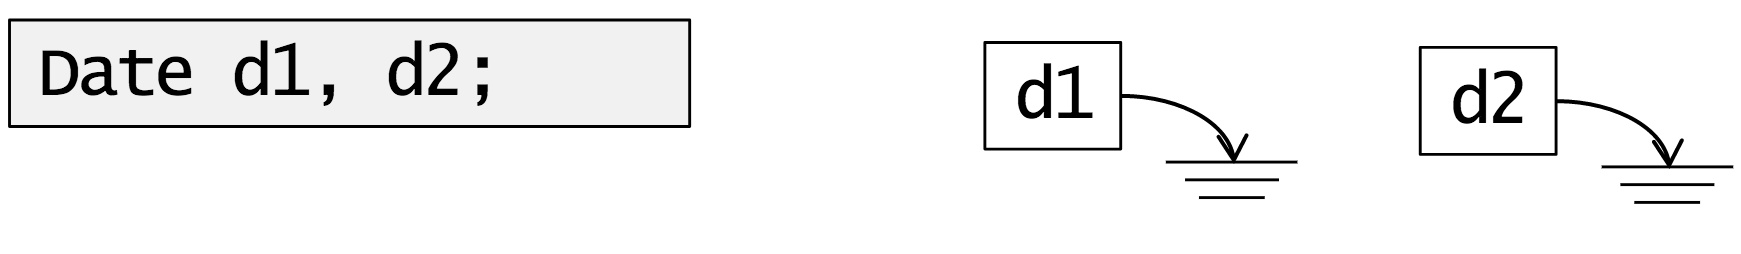
\includegraphics[width=.7\textwidth]{java/figures/basics/reference.png}
    \end{figure}
  \end{defn}
\end{defnbox}
\begin{notebox}[Note]\nospacing
  \begin{itemizenosep}
      \item Do not confuse C++ references with java references in Java variables are
  called (by convention) references.
      \item Reference variables are sort of C++ pointers but we can not do
    pointer arithmetic's on it e.g.\ \cppinline/ptr++/
      \item Reference Variables are of size:
    \begin{itemizenosep}
        \item 32-bit on a 32-bit JVM
        \item 32-bit or 64-bit on a 64-bit JVM, depending on the configuration
    \end{itemizenosep}
  \end{itemizenosep}
\end{notebox}
\begin{defnbox}\nospacing
  \begin{defn}[Static Type]\leavevmode
    A reference variable is declared to be of a specific type and that type,
    known as static type can never be changed.\leavevmode\\
    \ctr{Static type = type of reference variable}
  \end{defn}
\end{defnbox}
\begin{corbox}\nospacing
  \begin{cor}[Guarantees of Static Type]
    When a variable is declared as being of a particular type, then we have a
    language-enforced guarantee that any \textit{object} referenced by that
    reference variable will have (at least) all the features of that
    \textit{type}.\\
    $\Rightarrow$ \textit{dynamic type} needs to provide methods of \textit{static type}.
  \end{cor}  
\end{corbox}
\begin{defnbox}\nospacing
  \begin{defn}[Instanciation \javainline{new}]
    The new operator instantiates a class by dynamically allocating memory (=allocation at run time on the heap)
    for a new object and returns a reference to that memory.
    \begin{mintlinebox}{java}
      new MyClass();
    \end{mintlinebox}
    This reference can then be stored in/assigned to a (reference \cref{defn:referenceVariable}) variable.
    \begin{mintlinebox}{java}
      Type ref = new MyClass();
    \end{mintlinebox}
  \end{defn}
\end{defnbox}
\begin{notebox}[Note]\nospacing
  In Java, all class objects must be dynamically allocated.
\end{notebox}
%%% Local Variables:
%%% mode: latex
%%% TeX-master: "../../formulary"
%%% TeX-command-extra-options: "-shell-escape"
%%% End:
